\section{Introduction}
\label{sec:intro}

Pretrained Language Models (PLMs) are
large neural networks that are
used in a wide variety of NLP tasks. They operate under a
pretrain-finetune paradigm: models are first \emph{pretrained} over a large text corpus and then \emph{finetuned} on a downstream task. PLMs are thought of as good language encoders, supplying basic language understanding capabilities that can be used with ease for many downstream tasks.

A desirable property of a good language understanding model
is \emph{consistency}: the ability to make consistent
decisions in semantically equivalent contexts, reflecting a
systematic ability to generalize in the face of language variability.


Examples of consistency include: predicting the same answer in question answering and reading comprehension tasks regardless of paraphrase \cite{consistent-qa}; making consistent assignments in coreference resolution \cite{denis2009global,chang2011inference}; or making summaries factually consistent with the original document \cite{kryscinski2020evaluating}.
While consistency is important in many tasks, nothing in the training process explicitly targets it. One could hope that
the unsupervised training signal from large corpora
made available to PLMs such as BERT or RoBERTa
\cite{bert,roberta} is sufficient to induce consistency and
transfer it to downstream tasks.
In this paper, we show that this is not the case.



\begin{figure}[t!]
\centering

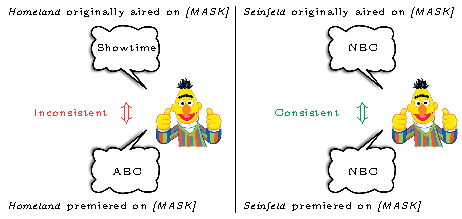
\includegraphics[width=1.\columnwidth]{figures/overview2}

\caption{Overview of our approach. 
We expect that a consistent model would predict the same answer for %every
 two paraphrases.
In this example, the model is inconsistent on the
\textit{Homeland} and consistent on the \textit{Seinfeld} paraphrases.}
\label{fig:overview}
% \vspace{-6mm}
\end{figure}


The recent rise of PLMs has sparked a discussion about whether these models can be used as Knowledge Bases (KBs) \cite{lama,petroni2020how,davison2019commonsense,peters2019knowledge,alpaqa,roberts2020much}. 
Consistency is a key property of KBs and is particularly important for automatically constructed KBs. %\nk{Not sure where to add this but we got the comment about answers that could change over time: president now vs past etc. KGs have the same problem. So it is reasonable to use the same setup.}
One of the biggest appeals of using a PLM as a KB is that we can
query it in natural language -- instead of relying on a specific KB schema.
The expectation is that PLMs abstract away from language and map queries in natural language into meaningful representations such that queries with identical intent but different language forms yield the same answer. 
For example, the query ``\textit{Homeland} premiered on \textit{[MASK]}'' should produce the same answer as ``\textit{Homeland} originally aired on \textit{[MASK]}''.
% \enote{hs}{this paragraph may suggest that PLM-KBs are not
%   consistent based on our results, but I don't think it is ever said? If that's
%   true, then it should be said}
Studying inconsistencies of PLM-KBs can also teach us about the organization of knowledge in the model or lack thereof. 
Finally, failure to behave consistently may point
to other representational issues such as the similarity between antonyms and synonyms \cite{nguyen2016integrating}, and overestimating events and actions (reporting bias) \cite{shwartz2020neural}.


In this work, we study the consistency of factual knowledge
in PLMs, \yenew{specifically in Masked Language Models (MLM) -- these are PLMs trained with the MLM objective \cite{bert,roberta}, as opposoed to other strategies such as standard language modeling \cite{gpt2} or text-to-text \cite{t5}. We ask:} Is the factual information we extract from PLMs invariant to paraphrasing? We use zero-shot evaluation since we want to inspect models directly, without adding biases through finetuning. This allows us to assess how much consistency was acquired during pretraining and to compare the consistency of different models. Overall, we find that the consistency of the PLMs we consider is poor, although there is a high variance between relations.



We introduce \resource{}, a new benchmark that enables us to measure consistency in PLMs (\S \ref{sec:probe}), by using factual knowledge that was found to be partially encoded in them \cite{lama,alpaqa}.
\resource{} is a manually curated resource
that provides patterns -- short textual prompts -- that are paraphrases of one another, with 328 paraphrases describing 38 binary relations such as \textit{X born-in Y}, \textit{X works-for Y} (\S \ref{sec:rel-graph}).
We then test multiple PLMs for knowledge consistency, i.e., whether
a model predicts the same answer for all patterns of a relation.
Figure \ref{fig:overview} shows an overview of our approach.
Using \resource{}, we probe for consistency in four PLM
types: BERT, BERT-whole-word-masking, RoBERTa and ALBERT (\S
\ref{sec:setup}).
Our experiments with \resource{} show that
current models have poor consistency, although with high variance between relations (\S \ref{sec:experiments}). 

Finally, we propose a method that improves model consistency
by introducing a novel consistency loss
(\S \ref{sec:adding_consistency}). We demonstrate that
trained with this loss, BERT achieves better consistency performance on unseen relations. However, more work is required to achieve fully consistent models.
